\documentclass[11pt]{article}

\usepackage{graphicx}
%\usepackage{algorithmic}
%\usepackage{algorithm}
\usepackage{amssymb}
\usepackage{amsmath}
\usepackage[mathscr]{euscript}

\begin{document}

\pagenumbering{arabic}

\begin{center}
{\LARGE{\textbf{Affective Computing}}} \\
\Large\textsc{Ph.D. Comprehensive Exam} \\[1em]
\large\textnormal{Mohammad Shayganfar - mshayganfar@wpi.edu} \\
\large\textnormal{May, 26 2015}
\end{center}

\section{Introduction to Affective Computing}

In this section, I discuss the concept of artificial emotions. I briefly review
the influential cognitive theories which describe emotions. These theories
provide cognitive structure of emotions and some of them describe the underlying
evaluative processes of emotion eliciting mechanisms. This is important in my
work because I am interested to investigate how emotions are involved in
collaboration and how the dynamics of a collaboration structure impact the
underlying processes of emotion.

Studies show that the decision making of
humans is not always logical \cite{GrossbergGutowski:affect-cognition}, and in
fact, not only is pure logic not enough to model human intelligence, but it also
shows failures when applied in artificial intelligence systems
\cite{dreyfus:artificial-critique}. Emotions impact fundamental parts of
cognition including perception, memory, attention and reasoning
\cite{clore:judgement-regulation}. This impact is caused by the information
emotions carry about the environment and event values. The influence of emotions
depends on an individual's focus of attention. For instance, a positive affect
can cause a positive attitude towards an object if the individual's focus is on
the object, whereas the same positive affect can be interpreted as a positive
feedback towards one's partner during the course of a collaboration. As another
example, a positive feedback can promote certain cognitive processes, or it can
inhibit other cognitive processes according to the conditions in the environment
\cite{clore:affective-guidance}. In both cases, emotions play a regulatory role
for cognitive processes \cite{gross:emotion-generation-regulation}. Some of the
effects flow from underlying shifts in the way people perceive and think under
the influence of emotion.

\section{Computational Theories of Emotion/Affect}

There are different types of computational theories of emotion. These theories
differ in type of relationships between their components and whether a
particular component play a cricual role in an individual emotion. For instance,
the basic component of an emotion can be the behavioral tendencies, cognitive
elements, or somatic processes. Emotion theories can also differ based on their
representationial distinction.

\subsection{Appraisal Theory}

The emotional experience is the experience of a particular situation
\cite{frijda:emotions}. Appraisal theory describes the cognitive process by
which an individual evaluates the situation in the environment with respect to
the individual's well-being and triggers emotions to control internal changes
and external actions. According to this theory, appraisals are separable
antecedents of emotion, that is, the individual first evaluates the environment
and then feels an appropriate emotion \cite{scherer:appraisal-processes}. The
appraisal procedure begins with the evaluation process of the environment
according to the internalized goals and is based on systematic assessment of
several elements \cite{scherer:sequential-appraisal-process}. The outcome of
this process triggers the appropriate emotions. In many versions of the
appraisal theory, appraisals also trigger cognitive responses often called
coping strategies. In fact, the coping mechanism manages the individual's
action with respect to the individual's emotional state and the existing
internal and/or external demands \cite{folkman:coping-pitfalls-promise}. The
large majority of computational models of emotions are based on this theory. An
individual can also use knowledge about the emotional reactions of others to
make inferences about them. According to the appraisal patterns, different
emotions can be experienced and expressed. Since expression of emotions reflects
one's intentions through the appraisal process, the \textit{reverse appraisal}
mechanism helps one to infer other's mental states based on their expressions.
\cite{gratch:reverse-appraisal, hareli:emotional-reaction-perception}.

Appraisal process is typically viewed as the cause of emotion and the cognitive
and behavioral changes associated with emotion. For instance, which particular
pattern of the appraisal variables (i.e., individual judgements) would elicit
certain emotion or an emotional expressions.\\

- List and brief description of appriasal variables.

\subsection{Dimensional Theories}

Dimensional theories of emotion argue that emotion should be conceptualized, as
points in a continuous (typically two or three) dimensional space rather than
looking at them as discrete entities (\cite{carver:affect-behavior},
\cite{mehrabian-russell:pad}, \cite{russell:core-affect},
\cite{watson:consensual-structure-mood}). Indeed, many dimensional theories
argue that discrete emotion categories (e.g., sadness, fear and anger) have no
``reality'' in that there are no specific brain regions or functions that
correspond to specific emotions \cite{barrett:emotions-natural}. Dimensional
theories do not emphasize the term emotion. Many computational dimensional
models build on the three dimensional “PAD” model of Mehrabian and Russell
\cite{mehrabian-russell:pad} where these dimensions correspond to pleasure (a
measure of valence), arousal (indicating the level of affective activation) and
dominance (a measure of power or control). Figure \ref{fig:pad} shows these
three dimensions.

\begin{figure}[tbh]
  \center
  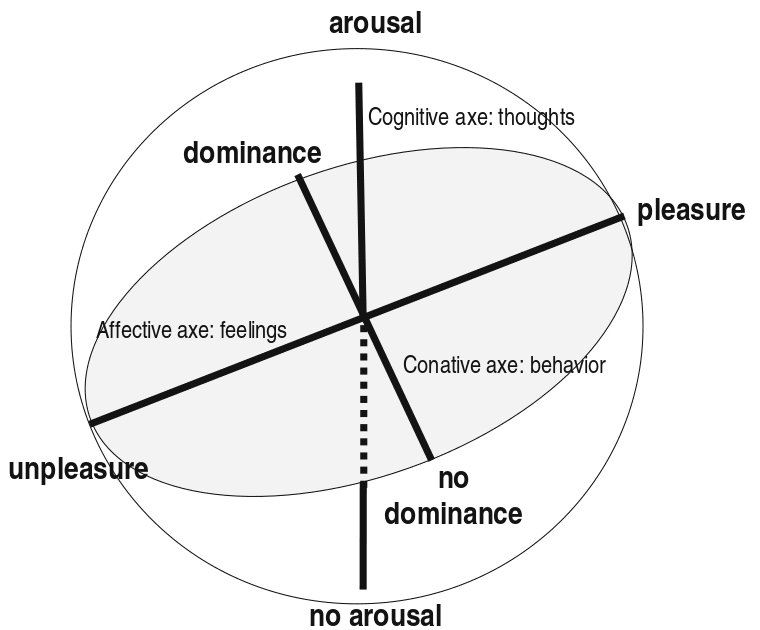
\includegraphics[width=.6\textwidth]{figure/dimensional2.png}
  \caption{Three dimensional model of pleasure, arousal and dominance as
  tripartite view of experience \cite{mehrabian:pad}.}
  \label{fig:pad}
\end{figure}

Dimensional models of emotion attempt to conceptualize human emotions by
defining where they lie in two or three dimensions. Some of the dimensional
models incorporate valence and arousal or intensity dimensions. These models
contrast theories of basic emotion, which propose that different emotions arise
from separate neural systems \cite{posner:circumplex-affect}. One of the
two-dimensional models that are most prominent is Russell's circumplex model
\cite{russell:circumplex-affect}.

\subsection{Other Approaches}

\subsubsection{Anatomic Approaches}

\subsubsection{rational Approaches}

\subsubsection{Communicative Approaches}

\section{Relation to Psychology and Sociology}

- Refer to functions of emotions (Page 48 in proposal).

\subsection{Emotion in Social Context}

Emotions are involved in developing social context. Humans are social and most
of the causations and constitutions of their emotions are social. Brian
Parkinson in \cite{parkinson:emotions-social} argues that many of the causes of
emotions are interpersonal and communicative rather than internal and reactive
phenomena. There are different social aspects of emotions influenced by various
factors such as social context and social relationship type. For instance, a
dominant-submissive social relationship can cause and contain different emotions
with different intensities compared to a reciprocal or a friendship social
relationship type. As another example, an emotion can be interpreted in a
certain way when an individual is situated in an environment with other people
who are expressing a particular emotion.

There are numerous ways that emotions can be
social \cite{tiedens:social-life}. There is a consensus on the fact that social
events and entities surrounding the individual play an essential role in the
generation of emotion. There are several ways in which other people elicit
emotional responses in us. One is that we feel the emotions of those around us.
Also, we have emotions about actions of those people around us. Another is we
have emotions about the things that happen to other people. Yet another is our
concern about our relationship with others that elicits emotion in us. The
groups to which we belong can also elicit our emotions. Moreover, we can feel
emotion about the success and failure of our own group or of other groups. In
addition, groups or individuals may make salient cultural concerns or societal
expectations that can elicit our emotions.

Beside the fact that social context can cause eliciting emotions in individuals,
social context provides information about what emotion should be expressed, by
whom, and in what situations. For instance, people are well aware of the
inappropriateness of expressing too much emotion to acquaintances
\cite{tiedens:social-life}. However, the social knowledge of emotion expression
is only partially delivered in an explicit fashion. There are studies on the
regulatory role of society and social relationships on emotions, showing that
people's emotions become socialized in implicit and unconscious ways. From this
perspective, social context can control and direct our attention toward certain
types of events and away from others.

\subsection{Social Meaning of Events}

Humans are emotional and social beings. Their emotions and the social context
in which they are involved have mutual impacts on each other. But, what if
humans can share their emotions with others just as they share their thoughts,
resources and their environment. Sharing an emotion with others may alter the
experience of an event. For instance, according to the nature of the
relationship between the individuals, the expression of emotions can either
restrain them from further interactions or improve their relationship.
Furthermore, individuals sharing emotions might possess a shared understanding
of their environment. Socially shared and regulated emotions also provide social
meanings to the events happening in the environment
\cite{wisecup:sociology-emotions}. For instance, people are likely to make
social inferences based on the presence or absence of particular emotions in
their social environment. Moreover, emotions can provide a basis for judgment
depending on the individual's relationships with others. In other words,
emotions can associate or disassociate an individual, therefore, they can change
or maintain the individual's social relationships \cite{tiedens:social-life}.

\subsection{Social Motivator}

Emotions can also play the role of a motivator in a social context. There is a
subset of social emotions delineated as role-taking emotions in
\cite{shott:emotion-social-life}. Shott provides two categories of
\textit{reflexive} (e.g. shame or pride) and \textit{empathic} (e.g., empathy or
pity) role-taking emotions. The reflexive emotions can motivate the individual's
self-control which depends on the anticipated reactions of others to the
individual's behaviors. For instance, guilt might lead the individual to behave
altruistically to restore a positive social stance for that individual. Empathic
or vicarious emotions are based on an individual mentally placing himself in
other's situation to understand how the other feels in that situation. These
emotions motivate prosocial behaviors to maintain an individual's internal
well-being \cite{thoits:socialogy-emotion}.

\subsection{Communicating Emotions}

Humans need to communicate their emotions within the social context
for different reasons. In \cite{goffman:self-presentation} Goffman argues that
human behaviors around others are performative which is often intended to convey
information to others. When human's actions are visible in the social context,
they behave differently in the presence of the others
\cite{zajonc:social-facilitation}. The social life of an individual is comprised
of the individual's internal cognitive competencies and his interactions in the
society. Lazarus says, if society is a fabric, then emotion is its color
\cite{lazarus:emotion-adaptation}. Although emotions undeniably have personal
aspects, they are usually experienced in a social context and acquire their
significance in relation to this context
\cite{parkinson:emotion-social-interaction}.

A successful and effective emotional communication necessitates ongoing
reciprocal adjustments between interactants that can happen by interpreting each
other's behaviors \cite{parkinson:emotion-social-interaction}. It not only
requires proper interpretation of the other's expressions, but also correct
assessment of the extent to which others can read an individual's expressions.
In emotional communication, individuals are constantly exchanging messages about
their mental states, and modifying each other's emotional responses as they
occur. Individuals perceive other's emotional states through verbal and
nonverbal responses during the interaction by processing relevant messages.
Communication dynamics represent the temporal relationship between these
communicative messages. The verbal and nonverbal messages from one participant
are better interpreted inside the correct context including the history and the
ongoing messages from the other individuals. Interpersonal dynamics (also known
as micro-dynamics in sociology) represent this influence of relationships
between individuals \cite{louis:communication-dynamic}.

\subsection{Social Functions}

Humans are able to communnicate their emotions in a social context. The social
functions of emotions are the reason behind why humans try to communicate their
emotions. In this section, I briefly discuss these social functions of emotions
since they are directly related to my work. Ekman in
\cite{ekman:argument-emotions} asserts that the primary function of emotions is
to mobilize the organism to deal with important interpersonal encounters. Darwin
in \cite{darwin:emotion-expression} argues the significance of social
communicative functions of emotions. Emotions describe interpersonal dynamics in
a way that they can constitute individuals' relationships
\cite{parkinson:emotions-social, tiedens:social-life}. One aspect of expressing
and communicating emotion in a social context is to express one's social motives
and intentions \cite{hess:darwin-emotion}. Another aspect of communicating
emotions is to reveal the underlying mental states of an individual
\cite{parkinson:emotion-communication}. In other words, emotions constitute two
different functionalities of expressing communicative signals associated with
one's social motives and intentions as well as expressing one's internal states
and how one feels about something. In \cite{kleef:emotion-regulate-social} Van
Kleef has discussed the idea of inferential processes with which individuals can
infer information about others' feelings, relational orientations and behavioral
intentions based on their emotional expressions. He also argues that emotional
expressions can impact social interactions by eliciting others' affective
responses.

Functional accounts vary according to the kind of system being analyzed.
Therefore, functional approaches to the emotions should vary by level of
analysis. Social functions of emotions can be analyzed in \textit{individual,
dyadic, group} and \textit{cultural} levels. My focus in this research is
on social functions in dyadic interaction (more specifically collaboration); I
also consider these functions at the individual's level especially when
interpreting the other collaborator's behaviors. Studies in all these levels
share a few assumptions about social accounts of emotions. They assume a)
individuals are social by nature and pursue solutions to survival problems in
social relationships, b) individuals apply their emotions to coordinate their
social interactions and relationships to address these survival problems, c)
emotions are processes mediating the individuals' relations to their dynamic
environment \cite{keltner:emotion-functions}. In dyadic interactions, studies
focus on how emotions impact the interactions of individuals in meaningful
relationships. In \cite{keltner:emotion-functions} Keltner and Haidt discuss
that in a dyadic setting, researchers mostly focus on communication of emotion
(e.g.\,Scherer \cite{scherer:vocal-expression}, DePaulo
\cite{depaulo:nonverbal-behavior}), properties (e.g.\,emotion contingency,
emotion synchrony) of dyadic emotions (e.g.\,Levenson \& Gottman
\cite{levenson:affective-exchange}), discourse (e.g.\,Bretherton
\cite{bretherton:emotions-functionalist}), and attachments (e.g. Hazan \& Shaver
\cite{hazan:emotion-attachment}).

\subsection{Dyadic Interaction}

As mentioned earlier, the social context is an important factor influencing
one's emotions. A dyadic interaction is one type of a setting in a social
context. Dyadic interaction tasks allow us to study emotion in a social setting
\cite{coan:emotion-dyadic}. Dyadic interaction tasks make it possible to examine
how individuals experience and express emotions during social interactions and
how emotions shape and are shaped by the reciprocal interactions between
individuals. In addition, eliciting and monitoring emotional processes yields
useful information about the role emotion plays in interpersonal relationships.
Compared with other emotion-eliciting events, events in a dyadic interaction can
better help us study an ongoing emotional relationship between two individuals
in addition to their internal emotional and cognitive processes. Dyadic
interaction tasks are ideal for studying a range of emotional responses because
of the fairly unstructured conversations between the individuals. Thus, dyadic
interaction tasks will generate a wide range of emotions in comparison with the
controlled emotion-eliciting events.

\section{Similarities and Differences}

- Rewrite this part [It is worth noting that there is a relationship between the
dimensions of core affect and appraisal dimensions – the pleasure dimension
roughly maps onto appraisal dimensions that characterize the valence of an
appraisal-eliciting event (e.g., intrinsic pleasantness or goal congruence),
dominance roughly map onto the appraisal dimension of coping potential, and
arousal a measure of intensity. However, they have quite different meaning:
appraisal is a relational construct characterizing the relationship between some
specific object/event and the individual’s beliefs desires and intentions and
several appraisals may be simultaneously active; core affect is a non-relational
construct summarizing a unique overall state of the individual.]

- Rewrite this part [Dimensional theories emphasize different components of
emotion than appraisal theories and link these components quite differently.
Dimensional theories foreground the structural and temporal dynamics of core
affect and often do not address affect’s antecedents in detail. Most
significantly, dimensional theorists question the tight causal linkage between
appraisal and emotion that is central to appraisal accounts. Dimensional
theorists conceive of core affect as a “non-intentional” state, meaning the
affect is not about some object (as in “I am angry at him). In such theories,
many factors may contribute to a change in core affect including symbolic
intentional judgments (e.g., appraisal) but also sub-symbolic factors such as
hormones and drugs (Schachter and Singer, 1962), but most importantly, the link
between any preceding intentional meaning and emotion is broken (as it is not
represented within core affect) and must be recovered after the fact, sometimes
incorrectly (Clore and Plamer, 2009, Clore et al., 1994). For example, Russell
argues for the following sequence of emotional components: some external event
occurs (e.g., a bear walks out of the forest), it is perceived in terms of its
affective quality; this perception results in a dramatic change in core affect;
this change is attributed to some “object” (e.g., the bear); and only then is
the object cognitively appraised in terms of its goal relevance, causal
antecedents and future prospects (see also, Zajonc, 1980).]

\section{Applications in Autonomous Agents and Robots}

There are several examples in artificial intelligence and robotics of applying
the appraisal theory as the basis of a computational model for emotions
\cite{adam:bdi-emotional-companion,kim:model-hri-appraisal,
marsella:ema-process-model}. In \cite{sander:systems-approach-appraisal} authors
describe a system approach to appraisal processes based on Scherer's work on
appraisal and the Component Process Model (CPM)
\cite{scherer:nature-function-emotion}. They show how the temporal unfolding
of emotions can be experimentally tested. In this thesis, I use the cognitive
appraisal theory of emotion provided by Gratch and Marsella in
\cite{gratch:domain-independent}. They lay out a general domain-independent
computational model of appraisal and coping. I use this appraisal approach,
in general, as an evaluation mechanism for the internal and external events to
assist the cognition and collaboration processes in my theory.

- Rewrite this [Computational dimensional models are most often used for
animated character behavior generation, perhaps because it translates emotion
into a small number of continuous dimensions that can be readily mapped to
continuous features of behavior such as the spatial extent of a gesture. For
example, PAD models describe all behavior in terms of only three dimensions
whereas modelers using appraisal models must either associate behaviors with a
larger number of appraisal dimensions (see Scherer and Ellgring, 2007, Smith and
Scott, 1997) or map appraisals into a small number of discrete, though perhaps
intensity-varying, expressions (Elliott, 1992). For a similar reason,
dimensional models also frequently used as a good representational framework for
systems that attempt to recognize human emotional behavior and there is some
evidence that they may better discriminate user affective states than approaches
that rely on discrete labels (Barrett, 2006).]

\subsection{Sociability}
Social skills have been mostly neglected in artificial intelligence and
robotics. However, there is a broad discussion in natural and social sciences,
e.g. psychology and primatology \cite{beheshtifar:social-intelligence-leadership,
bradberry:ability-skill-intelligence, keating:search-social-intelligence,
wexler:emotional-intelligence-appraisal, worden:primate-social-intelligence},
about the role of social factors in the development of intelligence
\cite{dautenhahn:social-autonomous-robots} (see Sections
\ref{section-emotion-social} to \ref{section-emotion-social-functions}). Robots
in the real world, e.g. domestic robots or collaborative robots, require
extensive understanding of aspects of humans' behaviors within their environment
as well as the ability to communicate and collaborate with them. Emotions, as
coordinated responses to detected or inferred relational meanings of the
environment (based on appraisal theory), can provide understanding of the social
environment, and the capability of communicating internal mental states and
maintaining collaborations with human partners. In fact, the emotion processes
momentarily respond to the unfolding affordances and constraints offered by the
dynamic context of a social interaction \cite{parkinson:holds-emotion}.
Appraisal can provide the assessment of goal relevance and goal congruence with
focus on self or other, the event, or the object in a social context
\cite{parrott:appraisal-social-emotions}. In short, the agent will be capable of
appraising the social environment in order to maintain effective social
interaction.

\subsection{Decision Making}

Decision-Making is an important and complicated process for any robot or virtual
agent. This process becomes more complicated when the agent needs to make a
decision considering its own private goal, the collaboration's shared goal and
the human collaborator's interests. I will provide more details about the
following concepts in Chapter \ref{chapter-theory}.

There are examples of rational and social agents designed based on the decision
theory and emotional states \cite{gmytrasiewicz:emotion-agent-decision}. Agents
must take a form of action after making a decision. Zhu and Thagard argue how
emotions significantly affect the action generation procedure as well as action
execution and control \cite{zhu:emotion-action}. The decision-making procedure,
as the basis of an agent's behaviors and actions, is a crucial process for an
agent in a social environment. Decision-making is a process that unfolds over
time and should be explored in more detail. According to
\cite{paulus:emotion-decision-belief}, the temporal structure of the
decision-making process contains three component processes:

\begin{enumerate}
  \item Choosing among options initially involves the process of
  \emph{assessing} the available options. One's affective state and appraisal
  evaluation of one's internal state as well as the surrounding environment
  helps in the assessment of all available options. For example, based on the
  scenario in section \ref{example-scenario}, Robot's emotion instance is fear
  because of an existing block in the plan and its evaluation of Astronaut's
  emotion as anger (for the same reason). The assessment of available options
  will be based on minimizing the distance to the shared goal and Astronaut's
  satisfaction. For instance, if Robot faces a non-critical task, it will give
  higher value to Astronaut's demanding task which will cause the postponement
  of its own.
  
  \item This process is followed by the \emph{selection} of an option based on
  the value that has been assigned to the option. This process is also augmented
  by affective evaluation of the world, including self, other(s) and the
  environment. For instance, in our scenario (see section
  \ref{example-scenario}), following the assessment of available options, Robot
  will focus on Astronaut's preferred task. Also, Robot creates and annotates
  meta information of the current state of the collaboration with affective
  evaluations.
  
  \item Finally, the outcome associated with the selected action is
  \emph{evaluated} and \emph{incorporated} into existing knowledge for
  subsequent decisions which implicitly and explicitly help the belief and
  appraisal emotion systems to operate coherently over time. For instance, if
  something goes wrong the Robot gives a negative affective attribution to the
  outcome of the selected action or even a certain path to that action to be
  used in future assessments.
\end{enumerate}

People's experience of events leak into their beliefs and ultimately decisions.
One aspect of these type of experiences is conscious or unconscious annotations
by different emotions. For instance, one will never forget working with a friend
due to the pleasant feeling of experiencing the outcome. On the other hand, a
person will always remember a particular experience in life because of an
utterly negative emotion that was felt at the time
\cite{paulus:emotion-decision-belief}.

Emotions appear to influence the value and weight computation of available
alternatives, and these computations are dynamically adjusted based on the
environment and the individual's internal states
\cite{pomerol:ai-decision-making}. This way agents can operate and take actions
based on preferences. In other words, emotional states of individuals are linked
to their decision-making processes, assuming that emotions affect the way gains
or losses are transformed to weights and values of the alternative beliefs,
actions, tasks, and, in general, plans \cite{paulus:emotion-decision-belief}.
The outcome of an action is also profoundly bound to the decision making process
as a final and an important stage. The experience of an outcome and in
particular, the differences between the expected and observed outcome provides
an opportunity to improve one's beliefs about consequences (value) of the
available alternatives and adopt a better decision policy in the future
\cite{pomerol:ai-decision-making, paulus:emotion-decision-belief}.

\section{Conclusion}

\bibliographystyle{plain}
\bibliography{mshayganfar}

\end{document}
